\documentclass[11pt]{extarticle}
\usepackage[T1]{fontenc}
\usepackage{amsmath}
\usepackage{amsthm}
\usepackage{amsfonts}
\usepackage{amssymb}
\usepackage{xcolor}	
\usepackage{graphicx}
\usepackage{caption}
\usepackage{subcaption}
\usepackage{multirow}
\usepackage{float}
\usepackage{enumitem}
\usepackage{titlesec}
%\usepackage{hyperref}

\usepackage{pdflscape}
\usepackage{fancyhdr}
\usepackage{booktabs}

% Show line numbers
\usepackage[mathlines]{lineno}
\renewcommand\linenumberfont{\normalfont\small\color{gray}}
% \linenumbers

% Show labels
% \usepackage{showlabels}

\numberwithin{equation}{section}
\usepackage{lipsum}
\setlength{\textwidth}     {16.0cm}
\setlength{\textheight}    {21.0cm}
\setlength{\evensidemargin}{ 0.0cm}
\setlength{\oddsidemargin} { 0.0cm}
\setlength{\topmargin}     {-0.5cm}
\setlength{\baselineskip}  { 0.7cm}


\newcommand{\R}{\mathbb{R}}
\newcommand{\D}{\mathbb{D}}
\newcommand{\C}{\mathbb{C}}
\newcommand{\N}{\mathbb{N}}
\newcommand{\Z}{\mathbb{Z}}
\newcommand{\dirichlet}{\mathcal{H}^2}

\theoremstyle{plain}
\newtheorem{example}{Example}[section]
\newtheorem{theorem}{Theorem}[section]
\newtheorem{corollary}{Corollary}[section]
\newtheorem{lemma}{Lemma}[section]
\newtheorem{proposition}{Proposition}[section]
\newtheorem{axiom}{Axiom}[section]
\newtheorem{remark}{Remark}[section]
\theoremstyle{definition}
\newtheorem{definition}{Definition}[section]
\newtheorem{assumption}{Assumption}
\renewcommand\theassumption{A\arabic{assumption}}
\newcommand{\expnumber}[2]{{#1}\mathrm{E}{#2}}


\begin{document}

\title{A Hardy space approximation supporting zero-free half-planes for the $\zeta$-function}

\author{
    Juan Manzur\thanks{Department of Mathematics,
    Universidad del Atlántico, Puerto Colombia, Atlántico, Colombia. email: jcmanzur@mail.uniatlantico.edu.co}
    \and
    Waleed Noor\thanks{Department of Mathematics,
    Institute of Mathematics, Statistics and Scientific Computing,
    State University of Campinas, CP 6065, 13081-970 Campinas
    SP, Brazil. email: waleed@unicamp.br}
    \and
    Gustavo Quintero\thanks{Department of Mathematics, Universidad del Atlántico, Puerto Colombia, Atlántico, Colombia. email: gdquintero@mail.uniatlantico.edu.co}
}

\date\today
\maketitle

\begin{abstract}
An equivalent version of the Báez-Duarte criterion \cite{baez} for the Riemann Hypothesis (RH) by Bagchi \cite{bagchi}  states that the RH holds true if and only if the function  $E(s) = 1/s$ belongs to the closed linear span of $G_k(s) = (k^{-s} - k^{-1})\zeta(s)/s,\, k \geq 2$ in the Hardy space \( H^2(\C_{1/2}) \), where $\C_{\alpha}$ denotes the half-plane $\mathrm{Re}(s)>\alpha$. We first show that if $E$ belongs to the closure of span$(G_k)_{k\geq 2}$ in \( H^2(\C_{\alpha}) \) for $\alpha>1/2$, then $\zeta$ is zero-free in $\mathbb{C}_\alpha$. We then use this as the basis for a numerical analysis of the sequence

\[
s_n = \left\| \sum_{k=2}^{n} \mu(k) G_k - E \right\|^2_\alpha,
\]
for $1/2\leq \alpha \leq 1$, where $\left\|.\right\|_\alpha$ is the norm in $H^2(\C_{\alpha})$ and $\mu$ the Möbius function.
 
\bigskip
\noindent
\textbf{Keywords:} Riemann hypothesis, zero-free half-planes, B\'aez-Duarte criterion, Hardy spaces, numerical approximation.
% \textbf{Keywords:} Riemann hypothesis, simulations, Nymann-Beurling.\\

% \noindent
% \textbf{Mathematics Subject Classification:} 90C30, 65K05, 49M37, 90C60, 68Q25.\\
\end{abstract}

\section{Introduction}

The Riemann Hypothesis (RH) asserts that all non-trivial zeros of the Riemann 
zeta function lie on the critical line $\mathrm{Re}(s) = \frac{1}{2}$. Its 
implications for the distribution of prime numbers make it one of the central 
open problems in mathematics.

A functional-analytic approach to RH was initiated by Nyman and Beurling, who 
showed that RH is equivalent to the density of a specific family of functions 
in $L^2(0,1)$~\cite{beurling,Nyman}. Báez-Duarte later refined this by 
replacing the original uncountable family with a countable sequence, simplifying 
the problem while preserving its essential structure~\cite{baez}. Balazard and 
Saias extended this approach to a weighted $\ell^2$-sequence space by posing the question of whether the orthogonal projection coefficients $c_{n,k}$ of $\mathbf{1}$ onto $\mathrm{span}\{r_k : 
2 \leq k \leq n\}$ satisfy
\[
\lim_{n\to\infty} c_{n,k} = -\frac{\mu(k)}{k}, \quad \forall\, k \geq 2,
\]
where $\mu$ is the Möbius function and $r_k(j) = j \bmod k$ denotes the 
remainder upon division of $j$ by $k$. This condition was shown by Weingartner in \cite{Weingartner} 
to be equivalent to the RH. This suggests that the choice of coefficients $\mu(k)/k$ (or $\mu(k)$ in our situation below after normalizing) is in a strict sense the best possible one.

A reformulation within the Hardy space $H^2(\mathbb{C}_{1/2})$ was established 
by Bagchi~\cite{bagchi}, where $\mathbb{C}_\alpha = \{s \in \mathbb{C} : \mathrm{Re}(s) > \alpha\}$ 
for $\alpha \in \mathbb{R}$: RH holds if and only if $E(s) = 1/s$ belongs to the 
closed linear span of
\[
G_k(s) = \bigl(k^{-s} - k^{-1}\bigr)\frac{\zeta(s)}{s}, \quad k \geq 1,
\]
in $H^2(\mathbb{C}_{1/2})$. Building on these ideas, Noor introduced an 
equivalent reformulation in the Hardy--Hilbert space $H^2(\mathbb{D})$ of the 
unit disk~\cite{waleed1}: RH holds if and only if the constant function 
$\mathbf{1}$ belongs to the closed linear span of
\[
h_k(z) = \frac{1}{1-z}\log\!\left(\frac{1+z+\cdots+z^{k-1}}{k}\right), \quad k \geq 2.
\]
In the same work, Noor established that the series $\sum_{k=2}^{\infty} 
\frac{\mu(k)}{k}(I-S)h_k$ converges to $1-z$ in $H^2(\mathbb{D})$, where 
$S$ is the shift operator. For an overview of the various equivalent reformulations of the Nyman-Beurling and Báez-Duarte approaches that appear in the literature, see \cite[p. 5-6]{noor-charles}.

The main idea of this paper is to generalize this 
result in an attempt to approximate RH using the reformulation of Bagchi in 
$H^2(\mathbb{C}_{1/2})$. To achieve this, we employ the Hilbert space of 
Dirichlet series $\mathcal{H}^2$, which presents a natural connection with 
the Hardy space of the disk. Within this framework, we construct a bounded 
operator $\mathcal{M}^\tau$ that establishes a connection between $\mathcal{H}^2$ 
and the Hardy spaces $H^2(\mathbb{C}_\alpha)$, leading to our main result 
(Theorem~\ref{main-teo}): the series $\sum_{k=2}^{\infty}\mu(k)G_k$ converges 
to $E$ in $H^2(\mathbb{C}_\alpha)$ for every $\alpha > 1$. Furthermore, 
Proposition~\ref{main-prop} establishes that for any $\alpha \geq 1/2$,
\[
E \in \overline{\mathrm{span}}\{G_k : k \geq 2\} \ \text{in } 
H^2(\mathbb{C}_\alpha) \implies \zeta(s) \neq 0, \quad \forall\, s \in \mathbb{C}_\alpha.
\]
An important question that arises is whether the convergence of the series 
extends to $1/2 \leq \alpha \leq 1$. Báez-Duarte~\cite{baez-unitary} showed 
that the $L^2$-analog of the sequence $s_n$ diverges in $L^2(0,1)$, which implies the divergence of $s_n$ itself
in $H^2(\mathbb{C}_{1/2})$. However, this does not discount the possibility of some subsequence of $s_n$ converging to $0$. In fact, the numerical evidence we present below strongly suggests that such subsequences exist. Studying the convergence in the range 
$1/2 < \alpha \leq 1$ is therefore essential, as it could provide information 
about zero-free regions of $\zeta$ within the critical strip, a problem that 
remains open and is widely considered to be as difficult as the RH itself.

The numerical analysis conducted in this work investigates the behavior of 
the partial sums
\[
s_n = \left\|\sum_{k=2}^{n}\mu(k)G_k - E\right\|^2_{H^2(\mathbb{C}_\alpha)}
\]
for $0.5 \leq \alpha \leq 1.0$. For $\alpha$ close to $1$, the sequence $s_n$ 
exhibits a clear decreasing trend, suggesting convergence in this region. 
For $\alpha$ close to $0.5$, the sequence shows persistent oscillations and 
significant deviations, indicating divergence consistent with the theoretical 
result of Báez-Duarte. Section~2 introduces the necessary function spaces and 
key results. Section~3 develops the main theoretical framework. Section~4 
presents the numerical experiments and their implications.

\section{Preliminaries}

We collect the function spaces and key results needed throughout the paper. The three Hilbert spaces $H^2(\mathbb{D})$, $\mathcal{H}^2$, and $H^2(\mathbb{C}_{1/2})$ are introduced here as the analytic framework within which the completeness conditions equivalent to the Riemann Hypothesis are formulated and studied.

\subsection{Hardy--Hilbert spaces and Dirichlet series}

Let $H^2(\mathbb{D})$ be the Hardy--Hilbert space of the unit disk, defined as
\[
H^2(\mathbb{D}) = \left\{ f(z) = \sum_{n=0}^{\infty} a_n z^n : \|f\|_{H^2}^2 = \sum_{n=0}^{\infty} |a_n|^2 < \infty \right\}.
\]
A recent reformulation of the RH, introduced in~\cite{waleed1}, is stated as follows. For each $k \geq 2$, define
\[
h_k(z) = \frac{1}{1-z} \log\!\left(\frac{1 + z + \cdots + z^{k-1}}{k}\right).
\]

\begin{theorem}[Theorem 6, \cite{waleed1}]
The Riemann Hypothesis holds if and only if the constant function $\mathbf{1}$ belongs to the closed linear span of $\{h_k : k \geq 2\}$ in $H^2(\mathbb{D})$.
\end{theorem}

Let $S = M_z$ denote the shift operator on $H^2(\mathbb{D})$, corresponding to multiplication by $z$. An additional result from~\cite{waleed1} plays a central role in this paper.

\begin{lemma}[Lemma 11, \cite{waleed1}]
\label{lem1:waleed}
The series $\sum_{k=2}^{\infty} \frac{\mu(k)}{k}(I - S)h_k$ converges to $1 - z$ in $H^2(\mathbb{D})$, where $\mu$ is the M\"{o}bius function.
\end{lemma}

Let $\mathcal{H}^2$ denote the Hilbert space of Dirichlet series, defined as
\[
\mathcal{H}^2 = \left\{ f(s) = \sum_{n=1}^{\infty} a_n n^{-s} : \|f\|_{\mathcal{H}^2}^2 = \sum_{n=1}^{\infty} |a_n|^2 < \infty \right\}.
\]
Setting $H^2_0(\mathbb{D}) = H^2(\mathbb{D}) \ominus \mathbb{C}$, there exists an isometric isomorphism
\[
\psi : H^2_0(\mathbb{D}) \longrightarrow \mathcal{H}^2, \qquad z^k \longmapsto k^{-s}.
\]


\subsection{The Hardy space of $\mathbb{C}_{1/2}$}

For $\alpha \in \mathbb{R}$, let $\mathbb{C}_\alpha = \{s = \sigma + it : \sigma > \alpha\}$ and let $H^2(\mathbb{C}_\alpha)$ denote the Hardy space of analytic functions $F$ on $\mathbb{C}_\alpha$ satisfying
\[
\|F\|^2_{H^2(\mathbb{C}_\alpha)} := \sup_{x > \alpha} \frac{1}{2\pi} \int_{-\infty}^{\infty} |F(x + it)|^2 \, dt < \infty.
\]
Any such $F$ admits a non-tangential boundary value $F^*$ almost everywhere on $\{\mathrm{Re}(s) = \alpha\}$, with
\[
\|F\|^2_{H^2(\mathbb{C}_\alpha)} = \frac{1}{2\pi}\int_{-\infty}^{\infty} |F^*(\alpha + it)|^2 \, dt.
\]
Moreover, $H^2(\mathbb{C}_\alpha)$ is a Hilbert space with reproducing kernel
\[
k_w(s) = \frac{1}{s + \overline{w} - 2\alpha}, \quad w \in \mathbb{C}_\alpha;
\]
in particular, convergence in norm implies pointwise convergence in $\mathbb{C}_\alpha$. 

Define the functions $G_k$ and $E$ in $H^2(\mathbb{C}_{1/2})$, for $k \geq 2$, as
\[
G_k(s) = (k^{-s} - k^{-1})\frac{\zeta(s)}{s} \quad \text{and} \quad E(s) = \frac{1}{s}.
\]
The Riemann Hypothesis reformulation for $H^2(\mathbb{C}_{1/2})$ can be stated as follows.

\begin{theorem}[Theorem 2, \cite{bagchi}]
RH is true if and only if $E$ belongs to the closed linear span of $\{G_k : k \geq 2\}$ in $H^2(\mathbb{C}_{1/2})$.
\end{theorem}

\section{An $H^2(\mathbb{C}_\alpha)$ approximation approach}

The main goal of this section is to show that $E$ belongs to the closed linear span 
of $\{G_k : k \geq 2\}$ in $H^2(\mathbb{C}_\alpha)$, for every $\alpha > 1$. 
For $\tau > 1/2$ and $k \geq 2$, define
\[
g_{k,\tau}(z) = k^{\tau-1}\sum_{n=1}^{\infty}\frac{z^n}{n^\tau} - \sum_{n=1}^{\infty}\frac{z^{nk}}{n^\tau}.
\]
It is clear that $g_{k,\tau} \in H^2_0$. Furthermore, we observe that
\begin{align*}
(\psi g_{k,\tau})(s) &= k^{\tau-1}\sum_{n=1}^{\infty}\frac{n^{-s}}{n^\tau} - k^{-s}\sum_{n=1}^{\infty}\frac{n^{-s}}{n^\tau}\\
&= (k^{\tau-1} - k^{-s})\zeta(s+\tau)\\
&= k^{\tau-1}f_{k,\tau} \quad \text{for } \mathrm{Re}(s) > 1/2,
\end{align*}
where $f_{k,\tau}(s) = (1 - k^{1-s-\tau})\zeta(s+\tau)$.

\subsection{A bounded operator from $\mathcal{H}^2$ to $H^2(\mathbb{C}_\alpha)$}

The operator $\mathcal{M}_{1/s} : \mathcal{H}^2 \to H^2(\mathbb{C}_{1/2})$, defined by 
$\mathcal{M}_{1/s} : f(s) \mapsto f(s)/s$, is bounded according to~\cite{6}. 
For $\tau \geq 1/2$, we extend this construction by defining 
$\mathcal{M}^\tau : \mathcal{H}^2 \to H^2(\mathbb{C}_{1/2+\tau})$ via $\mathcal{M}^\tau : f \longmapsto f(s - \tau)/s$. 
To see that $\mathcal{M}^\tau$ is well defined and bounded, note that for $\sigma > \tau + 1/2$,
\[
\frac{1}{2\pi}\int_{-\infty}^{\infty}\frac{|f(\sigma-\tau+it)|^2}{|\sigma+it|^2}\,dt
\leq \frac{1}{2\pi}\int_{-\infty}^{\infty}\frac{|f(\sigma-\tau+it)|^2}{|\sigma-\tau+it|^2}\,dt
= \|\mathcal{M}_{1/s}f\|^2_{H^2(\mathbb{C}_{1/2})},
\]
and taking the supremum over $\sigma > \tau + 1/2$ yields
\[
\|\mathcal{M}^\tau f\|_{H^2(\mathbb{C}_{1/2+\tau})} \leq \|\mathcal{M}_{1/s}\|\,\|f\|_{\mathcal{H}^2}, 
\qquad \forall f \in \mathcal{H}^2.
\]
The relevance of $\mathcal{M}^\tau$ to our approach lies in how it acts on the 
functions $1$ and $f_{k,\tau}$. A direct computation gives
\[
(\mathcal{M}^\tau 1)(s) = \frac{1}{s} = E(s),
\]
and
\[
(\mathcal{M}^\tau f_{k,\tau})(s) = \frac{f_{k,\tau}(s-\tau)}{s} 
= (1-k^{1-s})\frac{\zeta(s)}{s} = -kG_k(s).
\]

\subsection{Zero free region of $\zeta$ in $\mathbb{C}_\alpha$}

We now establish one of the main results of the paper. The key step is the following 
generalization of Lemma~\ref{lem1:waleed} to the family $\{g_{k,\tau}\}$.

\begin{lemma}\label{lem:main}
The series $\sum_{k=2}^{\infty} \frac{\mu(k)}{k^\tau} g_{k,\tau}$ converges 
to $-z$ in $H^2_0$, for each $\tau > 1/2$.
\end{lemma}

\begin{proof}
Note that
\begin{align*}
\sum_{k=2}^{n} \frac{\mu(k)}{k^\tau} g_{k,\tau}(z) 
&= \sum_{k=1}^{n} \frac{\mu(k)}{k^\tau} \left\{ k^{\tau-1}\sum_{j=1}^{\infty} \frac{z^j}{j^\tau} - \sum_{j=1}^{\infty}\frac{z^{jk}}{j^\tau} \right\}\\
&= \sum_{k=1}^{n} \frac{\mu(k)}{k} \sum_{j=1}^{\infty} \frac{z^j}{j^\tau} - \sum_{k=1}^{n} \frac{\mu(k)}{k^\tau} \sum_{j=1}^{\infty}\frac{z^{jk}}{j^\tau}.
\end{align*}
Since $\sum_{k=1}^{\infty} \frac{\mu(k)}{k} = 0$, the first term vanishes in the limit:
\[
\left\|\sum_{k=1}^{n} \frac{\mu(k)}{k} \sum_{j=1}^{\infty} \frac{z^j}{j^\tau}\right\|_{H^2_0} 
= \left|\sum_{k=1}^{n} \frac{\mu(k)}{k}\right| \left\|\sum_{j=1}^{\infty} \frac{z^j}{j^\tau}\right\|_{H^2_0} \longrightarrow 0.
\]
It therefore suffices to show that
\[
\left\| -\sum_{k=1}^{n} \frac{\mu(k)}{k^\tau} \sum_{j=1}^{\infty}\frac{z^{jk}}{j^\tau} + z \right\|_{H^2_0} \longrightarrow 0. \tag{3.1}
\]
A rearrangement of the double sum gives
\begin{align*}
\sum_{k=1}^{n} \frac{\mu(k)}{k^\tau} \sum_{j=1}^{\infty}\frac{z^{jk}}{j^\tau}
&= \sum_{j=1}^{n} \frac{z^j}{j^\tau}\left(\sum_{\substack{d|j,\\ 1\leq d\leq n}}\mu(d)\right) + \sum_{j=n+1}^{\infty} \frac{z^j}{j^\tau}\left(\sum_{\substack{d|j,\\ 1\leq d\leq n}}\mu(d)\right)\\
&= \sum_{j=1}^{n} \frac{z^j}{j^\tau}\left[\frac{1}{j}\right] + \sum_{j=n+1}^{\infty} \frac{z^j}{j^\tau}\left(\sum_{\substack{d|j,\\ 1\leq d\leq n}}\mu(d)\right), \tag{3.2}
\end{align*}
where the last equality uses the identity $\sum_{d|j}\mu(d) = \left[\frac{1}{j}\right]$. Returning to~(3.2),
\[
\sum_{k=1}^{n} \frac{\mu(k)}{k^\tau} \sum_{j=1}^{\infty}\frac{z^{jk}}{j^\tau} = z + \phi_n(z),
\]
where
\[
\phi_n(z) = \sum_{j=n+1}^{\infty} \left(\frac{1}{j^\tau}\sum_{\substack{d|j,\\ 1\leq d\leq n}}\mu(d)\right) z^j.
\]
It remains to show that $\|\phi_n\|_{H^2_0} \to 0$ as $n \to \infty$. 
Letting $\sigma(n)$ denote the number of divisors of $n$, we estimate
\[
\|\phi_n\|^2_{H^2_0} = \sum_{j=n+1}^{\infty} \frac{1}{j^{2\tau}}\left|\sum_{\substack{d|j,\\ 1\leq d\leq n}}\mu(d)\right|^2 
\leq \sum_{j=n+1}^{\infty} \frac{1}{j^{2\tau}}\left(\sum_{d|j}1\right)^2 
= \sum_{j=n+1}^{\infty} \frac{\sigma(j)^2}{j^{2\tau}}.
\]
Since $\sigma(n) = o(n^\epsilon)$ for every $\epsilon > 0$, choosing $\epsilon > 0$ 
such that $\tau > 1/2 + \epsilon$ yields
\[
\|\phi_n\|^2_{H^2_0} \lesssim \sum_{j=n+1}^{\infty} \frac{j^{2\epsilon}}{j^{2\tau}} 
= \sum_{j=n+1}^{\infty} \frac{1}{j^{2\tau - 2\epsilon}} \longrightarrow 0,
\]
since $2\tau - 2\epsilon > 1$.
\end{proof}

\begin{theorem}\label{main-teo}
The series $\sum_{k=2}^{\infty} \mu(k) G_k$ converges to $E$ in 
$H^2(\mathbb{C}_{1/2+\tau})$, for every $\tau > 1/2$.
\end{theorem}

\begin{proof}
By Lemma~\ref{lem:main} and the isomorphism $\psi$,
\[
\sum_{k=2}^{n} \frac{\mu(k)}{k} f_{k,\tau} \longrightarrow -1 \quad \text{in } \mathcal{H}^2.
\]
Applying $\mathcal{M}^\tau$ and using $(\mathcal{M}^\tau f_{k,\tau})(s) = -kG_k(s)$, we conclude
\[
\sum_{k=2}^{n} \mu(k) G_k \longrightarrow E \quad \text{in } H^2(\mathbb{C}_{1/2+\tau}). \tag{3.3}
\]
\end{proof}

\begin{corollary}\label{cor:main}
$E$ belongs to the closure linear span of $\{G_k : k \geq 2\}$ in 
$H^2(\mathbb{C}_\alpha)$, for every $\alpha > 1$.
\end{corollary}

As another consequence, Theorem~\ref{main-teo} yields a new proof of the 
non-vanishing of $\zeta$ in the half-plane $\mathbb{C}_1$.

\begin{proposition}\label{main-prop}
For any $\alpha \geq 1/2$,
\[
E \in \overline{\mathrm{span}}\{G_k : k \geq 2\} \ \text{in } H^2(\mathbb{C}_\alpha) 
\implies \zeta(s) \neq 0, \quad \forall s \in \mathbb{C}_\alpha.
\]
\end{proposition}

\begin{proof}
Let $\rho$ be a zero of $\zeta$ in $\mathbb{C}_\alpha$. Then $G_k(\rho) = 0$ 
for every $k \geq 2$. Since $H^2(\mathbb{C}_\alpha)$ is a reproducing kernel 
Hilbert space, convergence in norm implies pointwise convergence, so 
$E(\rho) = 0$, a contradiction.
\end{proof}

\section{Numerical evidence}

Theorem~\ref{main-teo} establishes that $\sum \mu(k)G_k$ converges to $E$ in
$H^2(\mathbb{C}_\alpha)$ for every $\alpha > 1$, while Proposition~\ref{main-prop}
shows that the membership of $E$ in the closed linear span of $\{G_k : k \geq 2\}$
forces $\zeta$ to be zero-free on $\mathbb{C}_\alpha$. The convergence is settled for $\alpha > 1$; the range
$1/2 \leq \alpha \leq 1$ (precisely the portion of the critical strip where
the behaviour of $\zeta$ is least understood) lies beyond the reach of our
analytical methods. The purpose of this section is to probe this range numerically.

We study the partial sums $ S_n = \sum_{k=2}^{n} \mu(k)G_k \in H^2(\mathbb{C}_\alpha)$,
and monitor the approximation error $s_n = \|S_n - E\|^2_{H^2(\mathbb{C}_\alpha)}$.
By Proposition~\ref{main-prop}, numerical evidence that $s_n \to 0$ for a given
$\alpha$ is evidence in favour of the non-vanishing of $\zeta$ on $\mathbb{C}_\alpha$.
At the opposite extreme, the $L^2(0,1)$-divergence established by
B\'aez-Duarte~\cite{baez-unitary} propagates to $s_n$ at $\alpha = 1/2$, so that
genuine convergence cannot be expected on the critical line itself. Our experiments
are accordingly designed to locate, as a function of $\alpha$, the transition
between these two regimes.

For a fixed $\alpha$, each error $s_n$ is obtained by numerically evaluating the
boundary integral that defines the $H^2(\mathbb{C}_\alpha)$ norm of $S_n - E$.
This integral was computed by adaptive Gauss--Kronrod quadrature (the QUADPACK
routine exposed through \texttt{scipy.integrate.quad}) in IEEE double precision,
with the Riemann zeta function obtained from its analytic continuation as
implemented in \texttt{scipy.special.zeta}. Starting from $S_2$, the partial sum
was extended one term at a time and the integral recomputed after each increment,
the iteration halting as soon as $s_n < \varepsilon$ or the prescribed time budget
was exhausted.

All computations were performed in Python~3.13 on a machine with a 5.2~GHz
Intel Core i9-12900K processor, 128~GB of DDR4 RAM, running Ubuntu~22.04~LTS.

% In this section, we analyze the numerical behavior of the partial sums $S_n = \sum_{k=2}^{n} \mu(k)G_k$ in $H^2(\mathbb{C}_\alpha)$ for different values of $\alpha$, measuring the 
% approximation error via $s_n = \|S_n - E\|^2_{H^2(\mathbb{C}_\alpha)}$. The goal is to examine whether $E$ belongs to the closed linear span of 
% $\{G_k : k \geq 2\}$, which by Proposition~\ref{main-prop} is a sufficient 
% condition for the non-vanishing of $\zeta$ in $\mathbb{C}_\alpha$. 

% All computations were performed in Python~3.12.7 on a machine with a 5.2~GHz 
% Intel Core i9-12900K processor, 128~GB DDR4 RAM, running Ubuntu~22.04.5~LTS.

\subsection{Experiments with tolerance and time}\label{subsec:tol}

Our first experiment quantifies how the rate of convergence of $(S_n)$ degrades
as $\alpha$ approaches the critical line. We discretised the interval $[0.5, 1.0]$
into $100$ equally spaced points,
\[
  \alpha_i = 0.5 + 0.005\,(i-1), \qquad i = 1, \ldots, 100,
\]
and, for three tolerance levels $\varepsilon \in \{10^{-2}, 10^{-3}, 10^{-4}\}$,
recorded for each $\alpha_i$ the smallest number of terms $n$ for which
$s_n < \varepsilon$, together with the time required to reach it. Here $\varepsilon$
fixes a prescribed accuracy of approximation, while $n$ serves as an intrinsic,
machine-independent measure of how rapidly $S_n$ approaches $E$: the larger the
$n$ needed to meet a fixed $\varepsilon$, the slower the convergence. To keep the
computation feasible, each run was capped at a time budget of $3600$ seconds;
when this limit was reached, the run was terminated and the largest $n$ attained
was recorded. The results are reported in Figure~\ref{fig:tolerance} and
Table~\ref{tab:tolerance}.

\begin{figure}[ht!]
\centering
\begin{tabular}{cc}
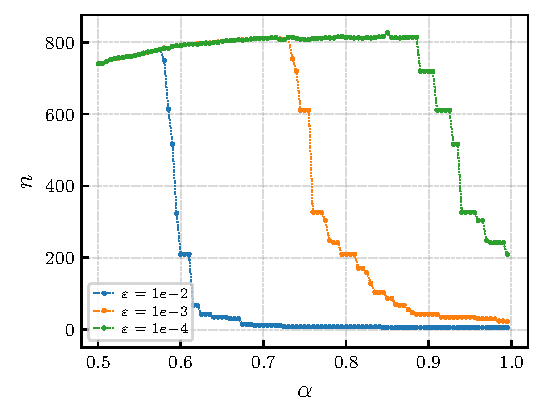
\includegraphics[scale=0.8]{alpha_vs_n.pdf} &
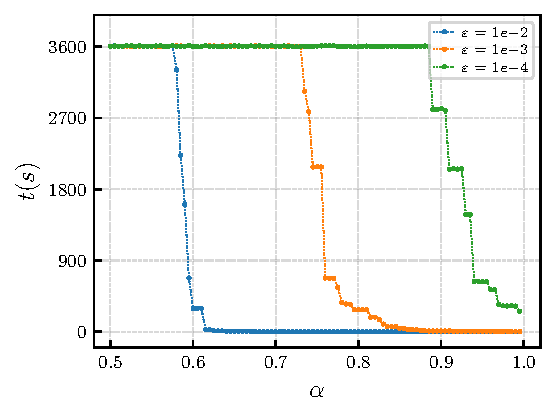
\includegraphics[scale=0.8]{alpha_vs_t.pdf} 
\end{tabular}
\caption{Tolerance test}
\label{fig:tolerance}
\end{figure}

\begin{table}[htb!]
\centering
\resizebox{0.5\textwidth}{!}{
\begin{tabular}{|c|cc|cc|cc|}
\hline
\multirow{2}{*}{$\alpha$} & 
\multicolumn{2}{c|}{$\varepsilon = \mathrm{1e{-}2}$} & 
\multicolumn{2}{c|}{$\varepsilon = \mathrm{1e{-}3}$} & 
\multicolumn{2}{c|}{$\varepsilon = \mathrm{1e{-}4}$} \\
\cline{2-7}
 & $n$ & Time (s) & $n$ & Time (s) & $n$ & Time (s) \\
\hline\hline
0.50 & 740 & $3.600\mathrm{e}{+3}$ & 740 & $3.600\mathrm{e}{+3}$ & 740 & $3.600\mathrm{e}{+3}$ \\
0.55 & 766 & $3.600\mathrm{e}{+3}$ & 766 & $3.600\mathrm{e}{+3}$ & 766 & $3.600\mathrm{e}{+3}$ \\
0.60 & 210 & $2.941\mathrm{e}{+2}$ & 791 & $3.600\mathrm{e}{+3}$ & 791 & $3.600\mathrm{e}{+3}$ \\
0.65 &  35 & $8.237\mathrm{e}{+0}$ & 803 & $3.600\mathrm{e}{+3}$ & 803 & $3.600\mathrm{e}{+3}$ \\
0.70 &  12 & $8.330\mathrm{e}{-1}$ & 811 & $3.600\mathrm{e}{+3}$ & 811 & $3.600\mathrm{e}{+3}$ \\
0.75 &   8 & $3.520\mathrm{e}{-1}$ & 611 & $2.084\mathrm{e}{+3}$ & 807 & $3.600\mathrm{e}{+3}$ \\
0.80 &   8 & $3.500\mathrm{e}{-1}$ & 210 & $2.792\mathrm{e}{+2}$ & 813 & $3.600\mathrm{e}{+3}$ \\
0.85 &   6 & $1.760\mathrm{e}{-1}$ &  87 & $4.466\mathrm{e}{+1}$ & 826 & $3.600\mathrm{e}{+3}$ \\
0.90 &   6 & $1.760\mathrm{e}{-1}$ &  43 & $1.057\mathrm{e}{+1}$ & 719 & $2.815\mathrm{e}{+3}$ \\
0.95 &   6 & $1.760\mathrm{e}{-1}$ &  35 & $6.988\mathrm{e}{+0}$ & 327 & $6.333\mathrm{e}{+2}$ \\
\hline
\end{tabular}
}
\caption{Corresponding to Figure~\ref{fig:tolerance}.}
\label{tab:tolerance}
\end{table}

A sharp, tolerance-dependent transition is evident. The coarse target
$\varepsilon = 10^{-2}$ is met for every $\alpha \geq 0.60$, requiring only six to
twelve terms once $\alpha \geq 0.70$. The intermediate target
$\varepsilon = 10^{-3}$ is met for $\alpha \geq 0.75$, and the fine target
$\varepsilon = 10^{-4}$ only for $\alpha \geq 0.90$; thus the threshold in
$\alpha$ below which the time budget is exhausted rises steadily as the demanded
accuracy increases. Below this transition the cost escalates abruptly, and for
$\alpha \leq 0.55$ none of the three tolerances is reached within the allotted
$3600$ seconds.

Two features of this transition deserve emphasis. First, Theorem~\ref{main-teo}
guarantees convergence of $S_n$ to $E$ only for $\alpha > 1$, yet the experiments
drive the error below $10^{-3}$ for $\alpha$ as small as $\approx 0.75$. The analytic threshold $\alpha > 1$ is therefore not
sharp, and the data support the expectation that convergence persists well into
the critical strip. Second, the failure to attain a prescribed tolerance at small
$\alpha$ must be read with care: it records a convergence rate that deteriorates
rapidly as $\alpha \to 1/2$, and is consistent with divergence. Disentangling these two readings near the endpoints is
the subject of the next subsection.

\subsection{Case studies at the endpoints $\alpha \approx 1/2$ and $\alpha \approx 1$}

The transition identified in Subsection~\ref{subsec:tol} separates two qualitatively
distinct regimes. To examine each in isolation, we refine the analysis near the
two endpoints of the interval. For $\alpha_{\min} \in \{0.5,\, 0.9\}$ we evaluate
$s_n$ on the grids
\[
  \alpha_i = \alpha_{\min} + 0.01\,i, \qquad i = 0, 1, \ldots, 9,
\]
at the sample points $n = 1000\,j$, $j = 1, \ldots, 100$, so that the behaviour of
$s_n$ is tracked up to $n = 10^5$. This larger range of $n$ lets the asymptotic
trend of each sequence emerge, beyond the onset captured by the tolerance
experiment of the previous subsection.

\begin{figure}[ht!]
    \centering
    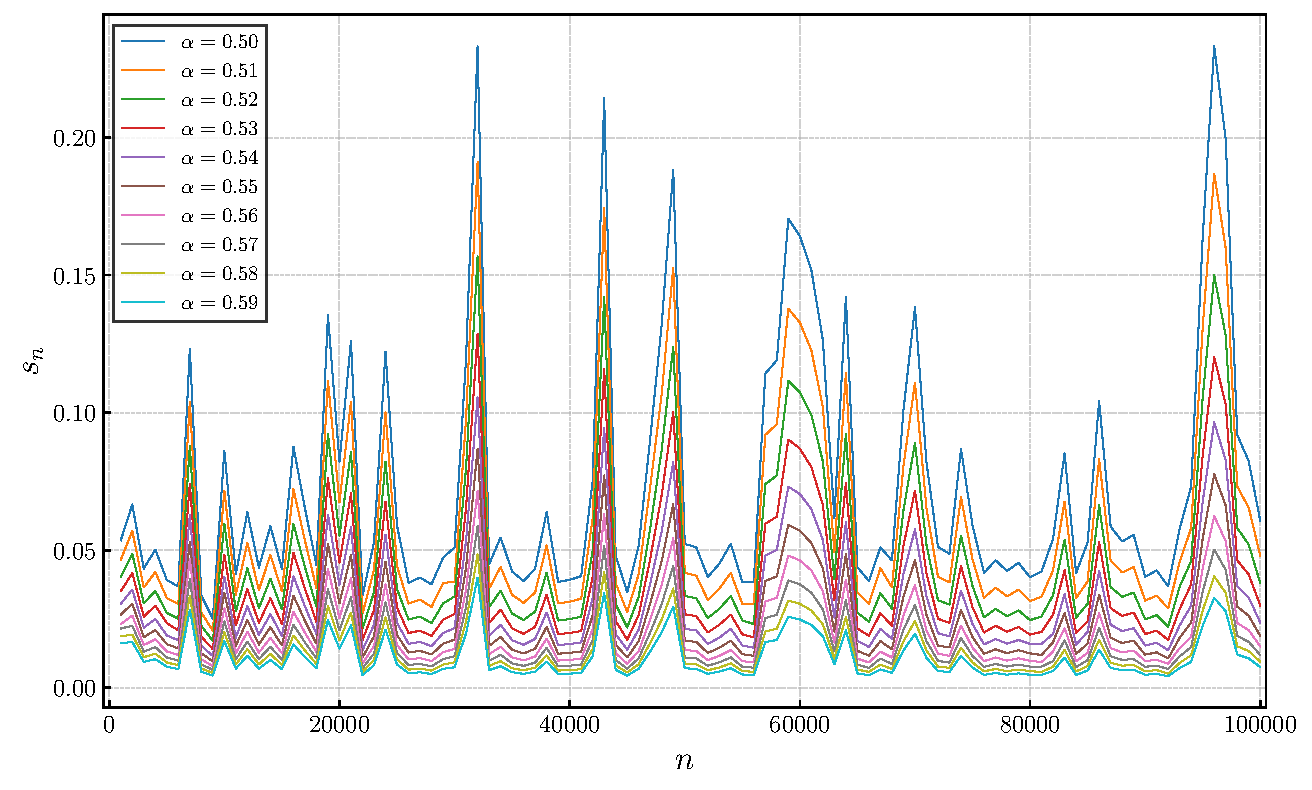
\includegraphics[scale=0.55]{alpha05.pdf}
    \caption{$0.50 \leq \alpha \leq 0.59$}
    \label{fig:alpha05}
\end{figure}

\begin{table}[ht!]
\centering
\resizebox{\textwidth}{!}{\begin{tabular}{|c|c|c|c|c|c|c|c|c|c|c|}
\hline
 \multirow{2}{*}{$n$} & \multicolumn{10}{c|}{$s_n$}\\
 \cline{2-11}
 & $\alpha = 0.50$ & $\alpha = 0.51$ & $\alpha = 0.52$ & $\alpha = 0.53$ & $\alpha = 0.54$ & $\alpha = 0.55$ & $\alpha = 0.56$ & $\alpha = 0.57$ & $\alpha = 0.58$ & $\alpha = 0.59$\\
 \hline\hline
1000   & $5.358\mathrm{e}{-2}$ & $4.651\mathrm{e}{-2}$ & $4.039\mathrm{e}{-2}$ & $3.510\mathrm{e}{-2}$ & $3.050\mathrm{e}{-2}$ & $2.655\mathrm{e}{-2}$ & $2.313\mathrm{e}{-2}$ & $2.155\mathrm{e}{-2}$ & $1.870\mathrm{e}{-2}$ & $1.625\mathrm{e}{-2}$ \\
10000  & $8.618\mathrm{e}{-2}$ & $7.170\mathrm{e}{-2}$ & $5.968\mathrm{e}{-2}$ & $4.836\mathrm{e}{-2}$ & $4.037\mathrm{e}{-2}$ & $3.461\mathrm{e}{-2}$ & $2.891\mathrm{e}{-2}$ & $2.417\mathrm{e}{-2}$ & $2.022\mathrm{e}{-2}$ & $1.692\mathrm{e}{-2}$ \\
20000  & $8.215\mathrm{e}{-2}$ & $6.742\mathrm{e}{-2}$ & $5.537\mathrm{e}{-2}$ & $4.549\mathrm{e}{-2}$ & $3.739\mathrm{e}{-2}$ & $3.077\mathrm{e}{-2}$ & $2.534\mathrm{e}{-2}$ & $2.089\mathrm{e}{-2}$ & $1.723\mathrm{e}{-2}$ & $1.421\mathrm{e}{-2}$ \\
30000  & $5.103\mathrm{e}{-2}$ & $3.865\mathrm{e}{-2}$ & $3.322\mathrm{e}{-2}$ & $2.682\mathrm{e}{-2}$ & $2.169\mathrm{e}{-2}$ & $1.753\mathrm{e}{-2}$ & $1.419\mathrm{e}{-2}$ & $1.149\mathrm{e}{-2}$ & $9.308\mathrm{e}{-3}$ & $7.468\mathrm{e}{-3}$ \\
40000  & $3.926\mathrm{e}{-2}$ & $3.131\mathrm{e}{-2}$ & $2.498\mathrm{e}{-2}$ & $1.994\mathrm{e}{-2}$ & $1.592\mathrm{e}{-2}$ & $1.272\mathrm{e}{-2}$ & $1.016\mathrm{e}{-2}$ & $8.060\mathrm{e}{-3}$ & $6.438\mathrm{e}{-3}$ & $5.149\mathrm{e}{-3}$ \\
50000  & $5.233\mathrm{e}{-2}$ & $4.180\mathrm{e}{-2}$ & $3.343\mathrm{e}{-2}$ & $2.674\mathrm{e}{-2}$ & $2.143\mathrm{e}{-2}$ & $1.716\mathrm{e}{-2}$ & $1.376\mathrm{e}{-2}$ & $1.103\mathrm{e}{-2}$ & $8.851\mathrm{e}{-3}$ & $7.112\mathrm{e}{-3}$ \\
60000  & $1.642\mathrm{e}{-1}$ & $1.328\mathrm{e}{-1}$ & $1.075\mathrm{e}{-1}$ & $8.699\mathrm{e}{-2}$ & $7.050\mathrm{e}{-2}$ & $5.715\mathrm{e}{-2}$ & $4.633\mathrm{e}{-2}$ & $3.762\mathrm{e}{-2}$ & $3.057\mathrm{e}{-2}$ & $2.486\mathrm{e}{-2}$ \\
70000  & $1.384\mathrm{e}{-1}$ & $1.110\mathrm{e}{-1}$ & $8.912\mathrm{e}{-2}$ & $7.162\mathrm{e}{-2}$ & $5.758\mathrm{e}{-2}$ & $4.633\mathrm{e}{-2}$ & $3.731\mathrm{e}{-2}$ & $3.009\mathrm{e}{-2}$ & $2.428\mathrm{e}{-2}$ & $1.960\mathrm{e}{-2}$ \\
80000  & $4.016\mathrm{e}{-2}$ & $3.152\mathrm{e}{-2}$ & $2.461\mathrm{e}{-2}$ & $1.933\mathrm{e}{-2}$ & $1.598\mathrm{e}{-2}$ & $1.253\mathrm{e}{-2}$ & $9.831\mathrm{e}{-3}$ & $7.715\mathrm{e}{-3}$ & $6.061\mathrm{e}{-3}$ & $4.762\mathrm{e}{-3}$ \\
90000  & $4.038\mathrm{e}{-2}$ & $3.171\mathrm{e}{-2}$ & $2.490\mathrm{e}{-2}$ & $1.955\mathrm{e}{-2}$ & $1.537\mathrm{e}{-2}$ & $1.208\mathrm{e}{-2}$ & $9.757\mathrm{e}{-3}$ & $7.671\mathrm{e}{-3}$ & $6.034\mathrm{e}{-3}$ & $4.750\mathrm{e}{-3}$ \\
100000 & $6.073\mathrm{e}{-2}$ & $4.805\mathrm{e}{-2}$ & $3.805\mathrm{e}{-2}$ & $2.996\mathrm{e}{-2}$ & $2.377\mathrm{e}{-2}$ & $1.887\mathrm{e}{-2}$ & $1.508\mathrm{e}{-2}$ & $1.191\mathrm{e}{-2}$ & $9.475\mathrm{e}{-3}$ & $7.543\mathrm{e}{-3}$ \\
\hline
\end{tabular}}
\caption{Corresponding to Figure~\ref{fig:alpha05}.}
\label{tab:alpha05}
\end{table}

\paragraph{The divergent regime $0.50 \leq \alpha \leq 0.59$.}
Figure~\ref{fig:alpha05} and Table~\ref{tab:alpha05} show that, across this entire
interval, $s_n$ exhibits prominent oscillations with no stabilising trend. Not
only does the sequence fail to decay, but even its local minima remain bounded
away from zero: at $\alpha = 0.50$ they hover near $4 \times 10^{-2}$ while the
peaks reach order $10^{-1}$, recurring without attenuation up to $n = 10^5$. This
is precisely the behaviour anticipated by theory. B\'aez-Duarte~\cite{baez-unitary}
proved that the $L^2(0,1)$ analogue of $s_n$ diverges, and this divergence
transfers to $H^2(\mathbb{C}_{1/2})$, so that $s_n \not\to 0$ at $\alpha = 1/2$.
The numerics show that this obstruction is robust throughout the lower edge of the
strip, and not confined to the critical line itself.

\paragraph{The convergent regime $0.90 \leq \alpha \leq 0.99$.}
Figure~\ref{fig:alpha09} and Table~\ref{tab:alpha09} reveal a markedly different
picture. The sequence $s_n$ now displays a clear overall decay, with oscillatory
peaks whose amplitude diminishes steadily as $n$ grows; although the decrease is
not strictly monotone, the envelope of the sequence contracts consistently. For
$\alpha = 0.99$, the error falls from $1.52 \times 10^{-4}$ at $n = 10^3$ to
$3.13 \times 10^{-6}$ at $n = 10^5$, a reduction of nearly two orders of magnitude,
and the same qualitative behaviour holds uniformly across the interval. These
observations strongly suggest that $S_n \to E$ in $H^2(\mathbb{C}_\alpha)$
throughout $0.90 \leq \alpha \leq 0.99$.

\begin{figure}[ht!]
    \centering
    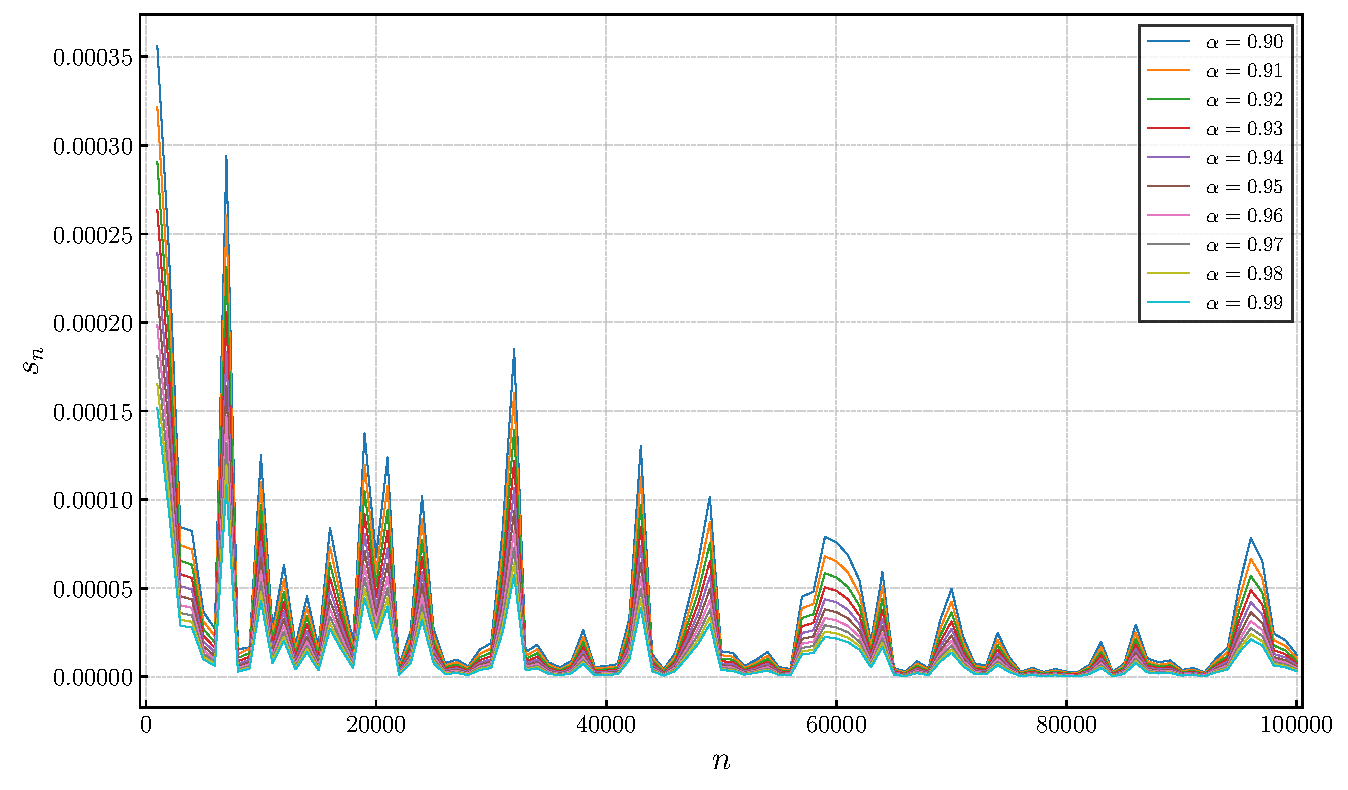
\includegraphics[scale=0.55]{alpha09.pdf}
    \caption{$0.90 \leq \alpha \leq 0.99$}
    \label{fig:alpha09}
\end{figure}

\begin{table}[ht!]
\centering
\resizebox{\textwidth}{!}{\begin{tabular}{|c|c|c|c|c|c|c|c|c|c|c|}
\hline
 \multirow{2}{*}{$n$} & \multicolumn{10}{c|}{$s_n$}\\
 \cline{2-11}
 & $\alpha = 0.90$ & $\alpha = 0.91$ & $\alpha = 0.92$ & $\alpha = 0.93$ & $\alpha = 0.94$ & $\alpha = 0.95$ & $\alpha = 0.96$ & $\alpha = 0.97$ & $\alpha = 0.98$ & $\alpha = 0.99$\\
 \hline\hline
1000   & $3.558\mathrm{e}{-4}$ & $3.215\mathrm{e}{-4}$ & $2.909\mathrm{e}{-4}$ & $2.636\mathrm{e}{-4}$ & $2.392\mathrm{e}{-4}$ & $2.177\mathrm{e}{-4}$ & $1.983\mathrm{e}{-4}$ & $1.812\mathrm{e}{-4}$ & $1.654\mathrm{e}{-4}$ & $1.516\mathrm{e}{-4}$ \\
10000  & $1.253\mathrm{e}{-4}$ & $1.100\mathrm{e}{-4}$ & $9.691\mathrm{e}{-5}$ & $8.562\mathrm{e}{-5}$ & $7.583\mathrm{e}{-5}$ & $6.707\mathrm{e}{-5}$ & $5.974\mathrm{e}{-5}$ & $5.335\mathrm{e}{-5}$ & $4.775\mathrm{e}{-5}$ & $4.297\mathrm{e}{-5}$ \\
20000  & $6.772\mathrm{e}{-5}$ & $5.882\mathrm{e}{-5}$ & $5.149\mathrm{e}{-5}$ & $4.498\mathrm{e}{-5}$ & $3.939\mathrm{e}{-5}$ & $3.463\mathrm{e}{-5}$ & $3.051\mathrm{e}{-5}$ & $2.699\mathrm{e}{-5}$ & $2.395\mathrm{e}{-5}$ & $2.133\mathrm{e}{-5}$ \\
30000  & $1.905\mathrm{e}{-5}$ & $1.594\mathrm{e}{-5}$ & $1.360\mathrm{e}{-5}$ & $1.164\mathrm{e}{-5}$ & $9.845\mathrm{e}{-6}$ & $8.498\mathrm{e}{-6}$ & $7.364\mathrm{e}{-6}$ & $6.408\mathrm{e}{-6}$ & $5.598\mathrm{e}{-6}$ & $4.909\mathrm{e}{-6}$ \\
40000  & $5.966\mathrm{e}{-6}$ & $5.138\mathrm{e}{-6}$ & $4.214\mathrm{e}{-6}$ & $3.460\mathrm{e}{-6}$ & $2.849\mathrm{e}{-6}$ & $2.350\mathrm{e}{-6}$ & $1.945\mathrm{e}{-6}$ & $1.616\mathrm{e}{-6}$ & $1.347\mathrm{e}{-6}$ & $1.127\mathrm{e}{-6}$ \\
50000  & $1.437\mathrm{e}{-5}$ & $1.215\mathrm{e}{-5}$ & $1.032\mathrm{e}{-5}$ & $8.802\mathrm{e}{-6}$ & $7.528\mathrm{e}{-6}$ & $6.473\mathrm{e}{-6}$ & $5.585\mathrm{e}{-6}$ & $4.839\mathrm{e}{-6}$ & $4.212\mathrm{e}{-6}$ & $3.683\mathrm{e}{-6}$ \\
60000  & $7.597\mathrm{e}{-5}$ & $6.516\mathrm{e}{-5}$ & $5.604\mathrm{e}{-5}$ & $4.854\mathrm{e}{-5}$ & $4.202\mathrm{e}{-5}$ & $3.650\mathrm{e}{-5}$ & $3.184\mathrm{e}{-5}$ & $2.781\mathrm{e}{-5}$ & $2.446\mathrm{e}{-5}$ & $2.157\mathrm{e}{-5}$ \\
70000  & $4.970\mathrm{e}{-5}$ & $4.245\mathrm{e}{-5}$ & $3.640\mathrm{e}{-5}$ & $3.125\mathrm{e}{-5}$ & $2.697\mathrm{e}{-5}$ & $2.335\mathrm{e}{-5}$ & $2.031\mathrm{e}{-5}$ & $1.772\mathrm{e}{-5}$ & $1.553\mathrm{e}{-5}$ & $1.367\mathrm{e}{-5}$ \\
80000  & $2.970\mathrm{e}{-6}$ & $2.375\mathrm{e}{-6}$ & $1.891\mathrm{e}{-6}$ & $1.509\mathrm{e}{-6}$ & $1.208\mathrm{e}{-6}$ & $9.647\mathrm{e}{-7}$ & $7.736\mathrm{e}{-7}$ & $6.219\mathrm{e}{-7}$ & $5.007\mathrm{e}{-7}$ & $4.044\mathrm{e}{-7}$ \\
90000  & $3.872\mathrm{e}{-6}$ & $3.146\mathrm{e}{-6}$ & $2.564\mathrm{e}{-6}$ & $2.095\mathrm{e}{-6}$ & $1.720\mathrm{e}{-6}$ & $1.416\mathrm{e}{-6}$ & $1.171\mathrm{e}{-6}$ & $9.733\mathrm{e}{-7}$ & $8.124\mathrm{e}{-7}$ & $6.820\mathrm{e}{-7}$ \\
100000 & $1.248\mathrm{e}{-5}$ & $1.051\mathrm{e}{-5}$ & $8.904\mathrm{e}{-6}$ & $7.568\mathrm{e}{-6}$ & $6.457\mathrm{e}{-6}$ & $5.534\mathrm{e}{-6}$ & $4.763\mathrm{e}{-6}$ & $4.117\mathrm{e}{-6}$ & $3.576\mathrm{e}{-6}$ & $3.125\mathrm{e}{-6}$ \\
\hline
\end{tabular}}
\caption{Corresponding to Figure~\ref{fig:alpha09}.}
\label{tab:alpha09}
\end{table}

We stress the conditional nature of this reading. By Proposition~\ref{main-prop},
genuine convergence $S_n \to E$ for such $\alpha$ would place $E$ in the closed
span of $\{G_k : k \geq 2\}$ and hence furnish a zero-free half-plane
$\mathbb{C}_\alpha$ deep within the critical strip, a conclusion lying far
beyond all currently known zero-free regions and widely regarded as being as
difficult as the Riemann Hypothesis itself. The evidence presented here is
therefore numerical and suggestive, not a proof. 

\clearpage

\begin{thebibliography}{99}
    \bibitem{apostol}
    T. M. Apostol, Introduction to analytic number theory. UTMS pringer, 1976.
	
	\bibitem{baez}
	L. Báez-Duarte, A strengthening of the Nyman-Beurling criterion for the Riemann hypothesis, Atti Acad. Naz. Lincei 14 (2003) 5-11.

    % \bibitem{BD_Arithmetical}

    % L, Baez-Duarte. Arithmetical Aspects of Beurling's Real Variable Reformulation of the Riemann Hypothesis. arXiv preprint math/0011254 (2000).
   \bibitem{baez-unitary}
  L. Báez-Duarte, A class of invariant unitary operators, Adv. Math., 144, No. 1 (1999), 1-12.

    \bibitem{Balazard}
    M. Balazard and E. Saias. Notes sur la fonction $\zeta$ de Riemann, 1. Adv. Math., Vol. 139 (1998) 310–321.
    
	
	\bibitem{bagchi}
	B. Bagchi, On Nyman, Beurling and Báez-Duarte's Hilbert space reformulation of the Riemann hypothesis, Proc. Indian Acad. Sci. Math. Sci. 116 (2) (2006) 137-146.

    \bibitem{beurling}
    A. Beurling, A closure problem related to the Riemann zeta-function. Proc. Nat. Acad. Sci., 41(5), 312-314, 1955.

    \bibitem{noor-charles}
    A. Ghosh, K. Kremnitzer, W. Noor, C. F. Santos, Zero-free half-planes of the $\zeta$-function via spaces of analytic functions, Adv. Math. 455 (2024) 109872.
	
	\bibitem{2}
	H. Hedenmalm, P. Lindqvist, K. Seip, A Hilbert space of Dirichlet series and systems of dilated functions in $L^{2}(0,1)$, Duke Math. J. 86 (1997) 1-37. MR 99i:42033.

    \bibitem{manzur-noor-santos}
    J. Manzur, S. W. Noor, and C. F. Santos. A weighted composition semigroup related to three open problems. J. Math. Anal. Appl. 525 (2023) 127261.
	
	
	%\bibitem{3}
	%N. Nikolski, In a shadow of the RH: cyclic vectors of the Hardy spaces on the Hilbert multidisc, Ann. Inst. Fourier 62 (5) (2012) 1601-1626.
	
	\bibitem{waleed1}
	S. W. Noor, A Hardy space analysis of the Báez-Duarte criterion for the RH, Adv. Math. 350 (2019) 242-255.

    \bibitem{Nyman}
      B. Nyman, On some groups and semigroups of translations. Thesis, Uppsala, 1950.

    \bibitem{6}
	H. Queffélec, K. Seip, Aproximation numbers of composition operators on the $H^{2}$ space of Dirichlet series, J. Funct. Anal. 268 (2015) 1612-1648.

      \bibitem{Weingartner}
    A. Weingartner. On a question of Balazard and Saias related to the Riemann hypothesis. Adv. Math. Vol. 208  (2007) 905–908. 
	
	
\end{thebibliography}


\end{document}